\section{Scalability and conflict-freedom}
\label{sec:scalability}

\XXX[STATUS]{Draft v4 ready.
  v4: Applied Eddie init-317-gdbaaa0d.
  v3: Moved back before the rule chapter.
  v2: Applied Frans init-154-g6dbae76.
  v1: New chapter vs SOSP.}

% \XXX[AC]{Should this go \emph{after} the rule chapter?  To show
%   commutative $\implies$ conflict-free and then conflict-free
%   $\implies$ scalable?  That might make it harder to add a discussion
%   of the converse and the effects of global clocks, but maybe that
%   should go in a separate ``Variants of the rule'' chapter after these
%   two?}

% Directory-based

% Interconnect

% cc-NUMA

% Should I explain cache coherence and directories and such here or
% assume that's understood?  How ``introductory'' should this chapter
% be?

% What really matters is what *doesn't* require coordination in the
% steady-state.  What can be done purely locally.  Any transition that
% involves coordination represents a scalability hazard.

Understanding multicore scalability requires first understanding the
hardware.
%
\Thiscref{sec:scalability} shows that, under
reasonable assumptions, conflict-free operations scale linearly on
modern multicore hardware.
%
The following \lcnamecref{sec:rule} will use conflict-freedom as a
stepping-stone in establishing the scalable commutativity rule.

% This result will act as the bridge from the formal connection between
% interface commutativity and conflict-free implementations established
% in the next chapter into the pragmatic realm of scalability.
% Together, these two results---formal and empirical---will form the
% scalable commutativity rule.


\subsection{Conflict-freedom and multicore processors}

The connection between conflict-freedom and scalability mustn't be taken
for granted.  Indeed, some early multi-processor architectures such as
the Intel Pentium depended on shared buses with global lock
lines~\cite[\S8.1.4]{intel-sdm-3}, so even conflict-free operations
did not scale.

Today's multicores avoid such centralized components.  Modern, large,
cache-coherent multicores utilize peer-to-peer interconnects between
cores and sockets; partition and distribute physical memory between
sockets (NUMA); and have deep cache hierarchies with per-core
write-back caches.
%
To maintain a unified, globally consistent view of memory despite
their distributed architecture, multicores depend on MESI-like
coherence protocols~\cite{papamarcos:mesi} to coordinate ownership of
cached memory.
%
A key invariant of these coherence protocols is that either a cache
line is not present in any cache, a mutable copy is present in a
single cache, or the line is present in any number of caches but is
immutable.
%
Maintaining this invariant requires coordination, and this is where
the connection to scalability lies.

\begin{figure}
  \centering
  \begin{tikzpicture}[x=2cm,y=2cm,bend angle=10,
%    every node/.style={draw},
    rfo/.style={->,red,ultra thick},
    local/.style={->,green!50!black,thick},
    remote/.style={->,dotted}]

    \begin{scope}[every node/.append style={shape=ellipse}]
      \node (I) at (90:1) {invalid};
      \node (S) at (200:1) {shared};
      \node (M) at (340:1) {modified};
    \end{scope}

    \begin{scope}[every node/.append style={shape=circle,inner sep=2pt}]
      \draw[rfo] (I) to[bend right] node[auto=right] {R} (S);
      \draw[rfo] (I) to[bend left] node[auto=left] {W} (M);

      \draw[rfo] (S) to[bend right] node[auto=right] {W} (M);
      \draw[local,<-] (S) to[loop left,distance=5mm] node {R} (S);
      \draw[remote] (S) to[bend right] node[auto=right] {rW} (I);

      \draw[local] (M) to[loop right,distance=5mm] node {R/W} (M);
      \draw[remote] (M) to[bend left] node[auto=left] {rW} (I);
      \draw[remote] (M) to[bend right] node[auto=right] {rR} (S);
    \end{scope}
  \end{tikzpicture}
  %
  \splitcaption{A basic cache-coherence state machine.}{``R'' and
    ``W'' indicate local read and write operations, while ``rR'' and
    ``rW'' indicate remote read and write operations.  Thick red lines
    show operations that cause communication.  Thin green lines show
    operations that occur without communication.}
  \label{fig:mesi}
\end{figure}

\Cref{fig:mesi} shows the basic state machine implemented by each
cache for each cache line.  This maintains the above invariant by
ensuring a cache line is either invalid in all caches, modified in one
cache and invalid in all others, or shared by any number of caches.
Practical implementations add further states---MESI's ``exclusive''
state, Intel's ``forward'' state~\cite{goodman:mesif}, and AMD's
``owned'' state~\cite[\S7.3]{amd-arch-2}---but these do not change the
basic communication required to maintain cache coherence.

Roughly, a set of operations scales when maintaining coherence does
not require communication in the steady state.
%
There are three memory access patterns that do not require
communication:
\begin{itemize}
\item
Multiple cores \emph{reading different} cache lines.  This scales
because, once each
cache line is in each core's cache, no further communication is
required to access it, so further reads can proceed independently of
concurrent operations.
%
\item
Multiple cores \emph{writing different} cache lines scales for much
the same reason.
%
\item
Multiple cores \emph{reading the same} cache line scales.
A copy of the line can be kept in each core's cache in shared mode,
which further reads from those cores can access without
communication.
\end{itemize}
%
That is, when memory accesses are conflict-free, they do no require
communication.
%
Furthermore, higher level operations composed of conflict-free reads
and writes are
themselves conflict-free and will also execute independently and in
parallel.
%
In all of these cases, conflict-free operations execute in the same
time in isolation as they do concurrently, so the total throughput of
$N$ such concurrent operations is proportional to $N$.
%
Therefore, given a perfect implementation of MESI, conflict-free
operations scale linearly.  The following sections verify this
assertion holds on real hardware under reasonable workload assumptions
and explore where it breaks down.


The converse is also true: conflicting operations cause
cache state transitions and the resulting coordination limits
scalability.
%
That is, if a cache line written by one core is read or written by
other cores, those operations must
coordinate and, as a result, will slow each other down.  While this
doesn't directly concern the scalable commutativity rule (which says
only when operations can be conflict-free, not when they must be
conflicted), the huge effect that conflicts can have on scalability
affirms the importance of conflict-freedom.  The following sections
also demonstrate the effect of conflicts on real hardware.

% The following sections verify that conflict-free operations scale
% linearly on real hardware, show that conflicts can severely limit
% scalability, and explore
% the practical limitations of conflict-free scalability.


\subsection{Conflict-free operations scale}
\label{sec:scalability:conflict-free}

We use two machines to evaluate conflict-free and conflicting
operations on real hardware: an 80-core (8 sockets $\times$ 10 cores)
Intel Xeon E7-8870 (the same machine used for evaluation in
\cref{sec:eval}) and, to show that our conclusions generalize, a
48-core (8 sockets $\times$ 6 cores) AMD Opteron 8431.
%
Both are cc-NUMA x86 machines with directory-based cache coherence,
but two manufacturers use different architectures, interconnects, and
coherence protocols.
%
\Cref{fig:machines} shows how the
two machines are broadly organized.

\begin{figure}
  \centering
  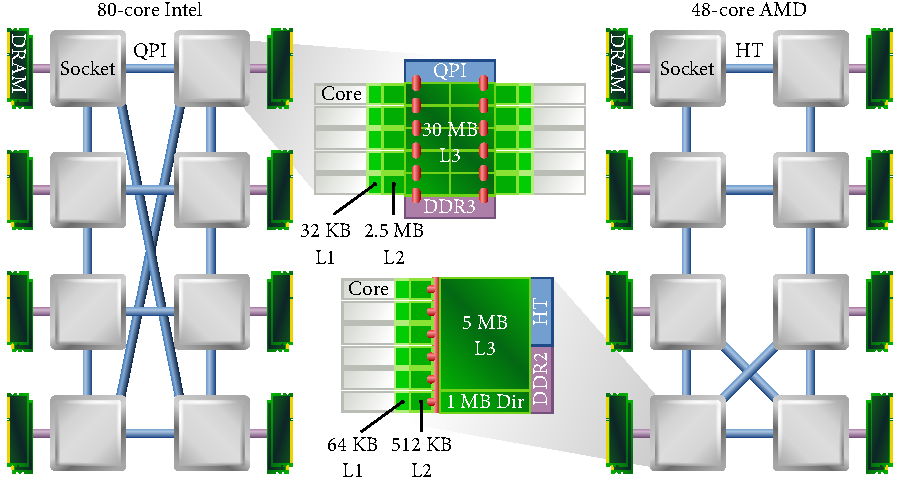
\includegraphics[width=\textwidth]{figures/machines.pdf}
  \caption[Organization of benchmark machines.]{Organization of Intel
    and AMD machines used for
    benchmarks~\cite{ben-motherboard,tom-motherboard-1,tom-motherboard-2}.}
  \label{fig:machines}
\end{figure}

\XXX[AC]{The conflict-free benchmarks wait between accesses.  Maybe
  they should be run at full tilt?}

\begin{figure}
  \centering
  \inputnodraft{graph/cfree-cycles}
  %
  \splitcaption{Conflict-free accesses scale.}{Each graph shows the
    cycles required to perform a conflict-free read or write from $N$
    cores.  Shading indicates the latency distribution for each $N$
    (darker shading indicates higher frequency).}
  \label{fig:cfree-cycles}
\end{figure}

\Cref{fig:cfree-cycles} shows the time required to perform
conflict-free memory accesses from varying numbers of cores.  The
first benchmark, shown in the top row of \cref{fig:cfree-cycles},
stresses read/read sharing by repeatedly reading the same cache line
from $N$ cores.  The latency of these reads remains roughly constant
regardless of $N$.
% (growing slightly on the AMD machine because of increasing noise).
After the first access from each core, the cache
line remains in each core's local cache, so later accesses occur
locally and independently, allowing read/read accesses to scale
perfectly.  Reads of different cache lines from different cores (not
shown) yield identical results to reads of the same cache line.

The bottom row of \cref{fig:cfree-cycles} shows the results of
stressing conflict-free writes by assigning each core a different
cache line and repeatedly writing these cache lines from each of $N$
cores.  In this case these cache lines enter a ``modified'' state at
each core, but then remain in that state, so as with the previous
benchmark, further writes can be performed locally and independently.
%
Again, latency remains constant regardless of $N$, demonstrating that
conflict-free write accesses scale.

\begin{figure}
  \centering
  \inputnodraft{graph/conflict-cycles}
  %
  \splitcaption{Conflicting accesses do not scale.}{Each graph shows
    the cycles required to perform a conflicting read or write from
    $N$ cores.  Shading indicates the latency distribution for each
    $N$ (estimated using kernel density estimation).}
  \label{fig:conflict-cycles}
\end{figure}

\Cref{fig:conflict-cycles} turns to the cost of conflicting
accesses.  The top row shows the latency of $N$ cores writing the same
cache line simultaneously.  The cost of a write/write conflict grows
dramatically as the number of writing cores increases because
ownership of the modified cache line must pass to each writing
core, one at a time.  On both machines, we also see a uniform
distribution of write latencies, which further illustrates this
serialization, as some cores acquire ownership quickly, while others
take much longer.

For comparison, a single complex system call like \code{open}
typically takes 1,000--2,000 cycles on these machines, while a single
conflicting write can take upwards of 50,000 cycles.
%
In the time it takes one thread to perform a single write to a highly
contended cache line, another could open 25 files.

% On the AMD machine, the growth of the mean latency and the spread of
% the distribution are noticeably super-linear as the benchmark adds
% cores further from core 0.

The bottom row of \cref{fig:conflict-cycles} shows the latency of $N$
cores simultaneously reading a cache line last written by core 0 (a
read/write conflict).  For the AMD machine, the results are nearly
identical to the write/write conflict case, since this machine
serializes requests for the cache line at CPU 0's socket.  On the
Intel machine, the cost of read/write conflicts also grows, albeit
more slowly, as Intel's architecture aggregates the read requests at
each socket.
%
We see this effect in the latency distribution, as well, with read
latency exhibiting up to eight different modes.  These modes reflect
the order in which the eight sockets' aggregated read requests are
served by CPU 0's socket.
% (notably, all sockets exhibit all modes, so this is not simply an
% effect of distance from the home socket).
Intel's optimization helps reduce the absolute
latency of reads, but nevertheless, read/write conflicts do not scale
on either machine.


\subsection{Limitations of conflict-free scalability}
\label{sec:scalability:limits}

Conflict-freedom is a good predictor of scalability on real hardware,
but it's not perfect.  Limited cache capacity and associativity cause
caches to evict cache lines (later resulting in cache
misses) even in the absence of coherence traffic.
%
And, naturally, a core's
very first access to a cache line will miss.  Such misses directly
affect sequential performance, but they may also affect the
scalability of conflict-free operations.
%
Satisfying a cache miss (due to conflicts or capacity) requires the
cache to fetch the cache line from another cache or from memory.
%
If this requires communicating with remote cores or remote memory, the
fetch may contend with concurrent operations for interconnect
resources or the remote memory controller.

Applications with good cache behavior are unlikely to exhibit such
issues, while applications with poor cache behavior usually have
sequential performance problems that outweigh scalability concerns.
Nevertheless, it's important to understand where our assumptions about
conflict-freedom break down.

\begin{figure}
  \centering
  \inputnodraft{graph/memscan}
  %
  \splitcaption{Operations scale until they exceed cache or directory
    capacity.}{Each graph shows the latency for repeatedly reading a
    shared region of memory (top) and writing separate per-core
    regions (bottom), as a function of region size and number of
    cores.}
  \label{fig:memscan}
\end{figure}

\Cref{fig:memscan} shows the results of a benchmark that explores some
of these limits by performing conflict-free accesses to regions of
varying sizes from varying numbers of cores.
%
This benchmark stresses the worst case: each core reads or writes in a
tight loop and all memory is physically allocated from CPU 0's socket,
so all misses contend for that socket's resources.
%
The top row of \cref{fig:memscan} shows the latency of reads to a
shared region of memory.
%
On both
machines, we observe slight increases in latency as the region exceeds
the L1 cache and later the L2 cache, but the operations continue to
scale until the region exceeds the L3 cache.  At this point the
benchmark becomes bottlenecked by the DRAM controller of CPU 0's
socket, so the reads no longer scale, despite being conflict-free.

We observe a similar effect for writes, shown in the bottom row of
\cref{fig:memscan}.  On the Intel machine, the operations scale until
the combined working set of the cores on a socket exceeds the socket's
L3 cache size.  On the AMD machine, we observe an additional
effect for smaller regions at high core counts: in this machine,
each socket has a 1~MB directory for tracking ownership of that
socket's physical memory, which this benchmark quickly exceeds.
% The Intel machine has a similar directory, but it's integrated into
% the L3~\cite{intel:e7-8870} and sufficiently provisioned even for
% this benchmark.

These benchmarks show some of the limitations to how far we can push
conflict-freedom before it no longer aligns with scalability.
Nevertheless, even in the worst cases demonstrated by these
benchmarks, conflict-free operations both perform and scale far better
than conflicted operations.

\XXX[AC]{False sharing is another common limitation.}


\subsection{Summary}

Despite some limitations, conflict-freedom is a good predictor
of linear scalability in practice.  Most software has good cache
locality and
high cache hit rates both because this is crucial for sequential
performance, and because it's in the interest of CPU manufacturers to
design caches that fit typical working sets.  For workloads that
exceed cache capacity, NUMA-aware allocation spreads physical memory
use across sockets and DRAM controllers, partitioning physical memory
access, distributing the DRAM bottleneck, and giving cores greater
aggregate DRAM bandwidth.

\Cref{sec:eval} will return to hard numbers on real hardware to show
that conflict-free implementations of commutative interfaces enable
software to scale not just at the level of memory microbenchmarks, but
at the level of an entire OS kernel and its applications.

% \XXX![FK]{Should this section cite some other performance studies?
%   E.g., ``these results are consistent with that other SOSP paper in
%   your session.''}  \XXX[AC]{I don't know how to compare them.}

% Causes home node access.  If the missing core is not the line's home
% node, then it has to make a remote request, which takes longer
% depending on how far away the remote node is and can contend for
% interconnect and the remote memory controller.  Even if a core
% misses on a local line, it may contend with other cores on the same
% node for resources.

% Assume some cache locality so compulsory misses are rare (enough to
% keep DRAM bandwidth demand within the capacity of the hardware),
% NUMA-aware memory allocation so that, when there is a miss, it can
% generally be serviced locally.  Such optimizations are standard
% practice, as they are important for sequential performance as they
% are for scalability.


% In the abstract model, two types of memory access scale:
% different cores reading the same read-only memory,
% and different cores writing distinct memory locations.
% Figure~\ref{fig:read-scaling} shows the costs of performing these two types of
% operations simultaneously from 6~cores, 24~cores, and 48~cores.  This benchmark
% stresses the worst case: all memory is physically allocated from NUMA node 0
% and each core reads or writes memory in a tight loop.  The behavior
% depends on how much memory is used by each core.  In both cases, the
% operations scale perfectly until the combined working set on a chip exceeds
% that chip's L3 cache.  After this, the benchmark is bottlenecked by
% node 0's DRAM controller, which can be saturated by even a single chip.  This
% indicates that physical hardware agrees with our abstract model for working sets
% that fit in cache.  Beyond this, hardware does not scale, though in practice
% NUMA-aware allocation and lower bandwidth requirements lessen the impact of
% overflowing the cache.
